\documentclass{article}
\usepackage[utf8]{inputenc}
\usepackage{graphicx}
\usepackage{float}
\usepackage{fancyhdr}
\usepackage{amsfonts}
\usepackage{amsmath}
\usepackage{amsthm}
\usepackage{amssymb}
\usepackage{enumitem}
\usepackage{verbatim}
\usepackage[
    letterpaper,
    margin=0.4in,
    tmargin=0.7in,
    bmargin=0.7in,
    headsep=12pt,
    footskip=12pt
]{geometry}

\theoremstyle{definition}
\newtheorem{ques}{Question}
\newtheorem*{ans}{Answer}

\renewcommand{\Re}{\operatorname{Re}}
\newcommand{\diam}{\operatorname{diam}}
\newcommand{\RR}{\mathbb{R}}

\pagestyle{fancy}
\fancyhf{}
\rhead{Control System Design}
\lhead{Matthew Stringer}
\chead{Problem Solutions}
\cfoot{\thepage}

\title{Control System Design Solutions}
\author{Matthew Stringer}
\date{}

\begin{document}
    \maketitle

    \section*{Chapter 2 Answers}
    \begin{ans}[2.5a]
        For each cart, we know that acceleration is equal to the net Force 
        divided by the mass. Thus,
        \begin{equation*}
            \ddot z_i = \frac{F_N}{M}.
        \end{equation*}
        We let the positive direction be to the right.
        Thus, 
        \begin{align*}
            \ddot z_1 = \frac{1}{M} \left( F_{m1} - F_s \right) \\
            \ddot z_2 = \frac{1}{M} \left( F_{m2} + F_s \right),
        \end{align*}
        where $F_{mi}$ are the forces from each respective motor, and
        $F_s$ is the force from the intermediate spring.
        Now lets derive the equations for the force $F_{mi}$.
        This will follow from Example 2B of the textbook.
        \begin{align*}
            e_i - v_i &= Ri_i \\
            e_i - K_2 w_i &= Ri \\
            \tau_i &= K_1 i_i \\
            e_i - K_2 w_i &= \frac{R\tau_i}{K_1} \\
            \tau_i &= \frac{K_1}{R}e_i - \frac{K_1 K_2}{R}w_i \\
            F_{mi} &= \frac{\tau_i}{r} = \frac{K_1}{rR}e_i - \frac{K_1 K_2}{rR}w_i \\
            w_i r &= \dot z_i \\
            F_{mi} &= \frac{K_1}{rR}e_i - \frac{K_1 K_2}{r^2 R}\dot z_i
        \end{align*}
        Now we will use Hooke's law to derive the force of the spring,
        \begin{equation*}
            F_s = kd = k(z_2 - z_1).
        \end{equation*}
        Thus, for our differential equations, we have
        \begin{align*}
            \ddot z_1 = \frac{k}{M} z_1 - \frac{k}{M}z_2 
            - \frac{K_1 K_2}{r^2 R M}\dot z_1 
            + \frac{K_1}{rRM} e_1
            \\
            \ddot z_2 = - \frac{k}{M} z_1 + \frac{k}{M}z_2 
            - \frac{K_1 K_2}{r^2 R M}\dot z_2 
            + \frac{K_1}{rRM} e_2.
        \end{align*}
        Finally for our state-space representation of the system, we have,
        \begin{align*}
            \begin{bmatrix}
                \dot z_1 \\
                \dot z_2 \\
                \ddot z_1 \\
                \ddot z_2 \\
            \end{bmatrix}
            =
            \begin{bmatrix}
                0 & 0 & 1 & 0 \\
                0 & 0 & 0 & 1 \\
                \frac{k}{M} & -\frac{k}{M} & -\frac{K_1 K_2}{r^2 R M} & 0 \\
                -\frac{k}{M} & \frac{k}{M} &  0 & -\frac{K_1 K_2}{r^2 R M} \\
            \end{bmatrix}
            \begin{bmatrix}
                z_1 \\
                z_2 \\
                \dot z_1 \\
                \dot z_2 \\
            \end{bmatrix}
            +
            \begin{bmatrix}
                0 & 0 \\
                0 & 0 \\
                \frac{K_1}{rRM} & 0 \\
                0 & \frac{K_1}{rRM} \\
            \end{bmatrix}
            \begin{bmatrix}
                e_1 \\ e_2
            \end{bmatrix}
            .
        \end{align*}
    \end{ans}
    \newpage
    \begin{ans}[2.5b]
        Using the differential equations above, we can create the
        following blcok diagram.
        \begin{figure}[H]
            \centering
            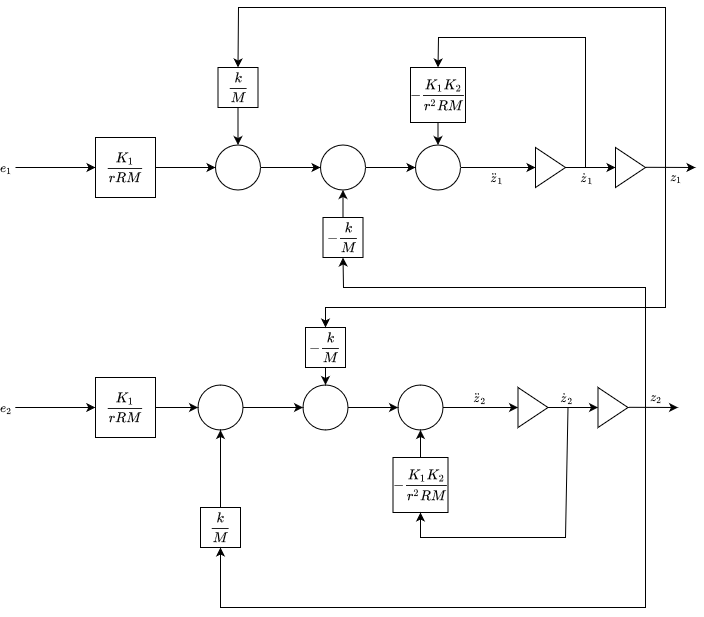
\includegraphics[height=5in]{Problem_2.5.png}
        \end{figure}
    \end{ans}

    \section*{Chapter 5 Answers}
    \begin{ans}[5.2a]
        Removing the motor from the left most cart results
        in the following differential equations.
        \begin{align*}
            \ddot z_1 = \frac{1}{M} \left( - F_s \right) \\
            \ddot z_2 = \frac{1}{M} \left( F_{m2} + F_s \right),
        \end{align*}
        Thus, the differential equations become
        \begin{align*}
            \ddot z_1 &= -\frac{k}{M} z_1 + \frac{k}{M} z_2 \\
            \ddot z_2 &= - \frac{k}{M} z_1 + \frac{k}{M}z_2 
            - \frac{K_1 K_2}{r^2 R M}\dot z_2 
            + \frac{K_1}{rRM} e_2.
        \end{align*}
        Thus, the state space system becomes
        \begin{align*}
            \begin{bmatrix}
                \dot z_1 \\
                \dot z_2 \\
                \ddot z_1 \\
                \ddot z_2 \\
            \end{bmatrix}
            =
            \begin{bmatrix}
                0 & 0 & 1 & 0 \\
                0 & 0 & 0 & 1 \\
                \frac{k}{M} & -\frac{k}{M} & 0 & 0 \\
                -\frac{k}{M} & \frac{k}{M} &  0 & -\frac{K_1 K_2}{r^2 R M} \\
            \end{bmatrix}
            \begin{bmatrix}
                z_1 \\
                z_2 \\
                \dot z_1 \\
                \dot z_2 \\
            \end{bmatrix}
            +
            \begin{bmatrix}
                0 \\
                0 \\
                0 \\
                \frac{K_1}{rRM} \\
            \end{bmatrix}
            e_2
            .
        \end{align*}
        Recall that in order for the system to be controllable,
        the matrix 
        \begin{equation*}
            Q = 
            \begin{bmatrix}
                B & AB & A^2 B & A^3 B
            \end{bmatrix}
        \end{equation*}
        must have rank 4.
        \begin{comment}
% Matlab LiveScript:
syms k M K1 K2 r R
A = [
0 0 1 0
0 0 0 1
k/M -k/M 0 0
-k/M k/M 0 -K1*K2/(r^2*R*M)
];

B = [
    0 
    0 
    0
    K1/(r*R*M)
    ];
Q = [B A*B A^2*B A^3*B] 
rank(Q)
        \end{comment}
        Using matlab, we find that
        \begin{equation*}
            \begin{array}{l}
                Q = 
                \left(\begin{array}{cccc}
                0 & 0 & 0 & \sigma_2 \\
                0 & \sigma_3  & \sigma_1  & \sigma_4 \\
                0 & 0 & \sigma_2  & \frac{{K_1 }^2 \,K_2 \,k}{M^3 \,R^2 \,r^3 }\\
                \sigma_3  & \sigma_1  & \sigma_4  & -\frac{K_1 \,{\left(\frac{K_1 \,K_2 \,k}{M^2 \,R\,r^2 }+\frac{K_1 \,K_2 \,\sigma_5 }{M\,R\,r^2 }\right)}}{M\,R\,r}
                \end{array}\right)\\
                \mathrm{}\\
                \textrm{where}\\
                \mathrm{}\\
                \;\;\sigma_1 =-\frac{{K_1 }^2 \,K_2 }{M^2 \,R^2 \,r^3 }\\
                \mathrm{}\\
                \;\;\sigma_2 =-\frac{K_1 \,k}{M^2 \,R\,r}\\
                \mathrm{}\\
                \;\;\sigma_3 =\frac{K_1 }{M\,R\,r}\\
                \mathrm{}\\
                \;\;\sigma_4 =\frac{K_1 \,\sigma_5 }{M\,R\,r}\\
                \mathrm{}\\
                \;\;\sigma_5 =\frac{k}{M}+\frac{{K_1 }^2 \,{K_2 }^2 }{M^2 \,R^2 \,r^4 }
            \end{array}
        \end{equation*}
        Also using matlab, we find that the rank of this matrix is 4.
        Thus, the system is controllable.
    \end{ans}
    \begin{ans}[5.2b]
        Recall the state space system from problem 2.5
        \begin{align*}
            \begin{bmatrix}
                \dot z_1 \\
                \dot z_2 \\
                \ddot z_1 \\
                \ddot z_2 \\
            \end{bmatrix}
            =
            \begin{bmatrix}
                0 & 0 & 1 & 0 \\
                0 & 0 & 0 & 1 \\
                \frac{k}{M} & -\frac{k}{M} & -\frac{K_1 K_2}{r^2 R M} & 0 \\
                -\frac{k}{M} & \frac{k}{M} &  0 & -\frac{K_1 K_2}{r^2 R M} \\
            \end{bmatrix}
            \begin{bmatrix}
                z_1 \\
                z_2 \\
                \dot z_1 \\
                \dot z_2 \\
            \end{bmatrix}
            +
            \begin{bmatrix}
                0 & 0 \\
                0 & 0 \\
                \frac{K_1}{rRM} & 0 \\
                0 & \frac{K_1}{rRM} \\
            \end{bmatrix}
            \begin{bmatrix}
                e_1 \\ e_2
            \end{bmatrix}
            .
        \end{align*}
        In order for this system to be controllable, 
        the rank of  
        \begin{equation*}
            Q = 
            \begin{bmatrix}
                B & AB & A^2 B & A^3 B
            \end{bmatrix}
        \end{equation*}
        must be 4.
        By using matlab, we can find
        \begin{comment}
% Matlab LiveScript:
syms k M K1 K2 r R
A = [
0 0 1 0
0 0 0 1
k/M -k/M -K1*K2/(r^2*R*M) 0
-k/M k/M 0 -K1*K2/(r^2*R*M)
];

B = [
    0 0 
    0 0 
    K1/(r*R*M) 0
    0 K1/(r*R*M)
    ];
Q = [B A*B A^2*B A^3*B] 
rank(Q)
        \end{comment}
        \begin{equation*}
            \begin{array}{l}
            Q = 
                \left(\begin{array}{cccccccc}
                0 & 0 & \sigma_4  & 0 & \sigma_1  & 0 & \sigma_5  & \sigma_2 \\
                0 & 0 & 0 & \sigma_4  & 0 & \sigma_1  & \sigma_2  & \sigma_5 \\
                \sigma_4  & 0 & \sigma_1  & 0 & \sigma_5  & \sigma_2  & \sigma_6  & \sigma_3 \\
                0 & \sigma_4  & 0 & \sigma_1  & \sigma_2  & \sigma_5  & \sigma_3  & \sigma_6 
                \end{array}\right)\\
                \mathrm{}\\
                \textrm{where}\\
                \mathrm{}\\
                \;\;\sigma_1 =-\frac{{K_1 }^2 \,K_2 }{M^2 \,R^2 \,r^3 }\\
                \mathrm{}\\
                \;\;\sigma_2 =-\frac{K_1 \,k}{M^2 \,R\,r}\\
                \mathrm{}\\
                \;\;\sigma_3 =\frac{2\,{K_1 }^2 \,K_2 \,k}{M^3 \,R^2 \,r^3 }\\
                \mathrm{}\\
                \;\;\sigma_4 =\frac{K_1 }{M\,R\,r}\\
                \mathrm{}\\
                \;\;\sigma_5 =\frac{K_1 \,\sigma_7 }{M\,R\,r}\\
                \mathrm{}\\
                \;\;\sigma_6 =-\frac{K_1 \,{\left(\frac{K_1 \,K_2 \,k}{M^2 \,R\,r^2 }+\frac{K_1 \,K_2 \,\sigma_7 }{M\,R\,r^2 }\right)}}{M\,R\,r}\\
                \mathrm{}\\
                \;\;\sigma_7 =\frac{k}{M}+\frac{{K_1 }^2 \,{K_2 }^2 }{M^2 \,R^2 \,r^4 }
                \end{array}
        \end{equation*}
        Also using matlab, we find that the rank of this matrix is always 4.
    \end{ans}
\end{document}